%%=============================================================================
%% Uitwerking
%%=============================================================================

\chapter{Uitwerking}
\label{ch:uitwerking}


\section{Benodigdheden}
\label{sec:Benodigdheden}

\subsection{Data}
Een onmisbaar onderdeel om aan machine learning te doen is uiteraard de data. Tijdens de eerste fases van het project wordt er gebruik gemaakt van zelf gegenereerde data in Excel. De data die uit de arcademachine ontvangen zal worden zal in CSV-formaat zijn. Doordat Excel-tabbladen opgeslagen kunnen worden in een CSV-file is dit dan ook een logische keuze. 
Er zullen zo'n 500 metingen beschikbaar zijn die kunnen ingelezen worden in het programma. 

We willen uiteraard weten hoe goed het algoritme scoort dit kunnen we testen door testdata te voorzien. De dataset die we uit Excel halen zal opgesplitst worden in trainingsdata en testdata. Het algoritme zal met de trainingsdata een hypothese vormen die ervoor zal zorgen dat ook nieuwe of nog ongekende data een goede voorspelling krijgt. Daarom is het belangrijk om een dataset te hebben die data bevat die nog niet eerder gebruikt is door het algoritme. Enkel op deze manier kunnen we zeker zijn dat het algoritme een goede hypothese heeft gemaakt. Als testdata nemen we 20\% van de hele dataset. 

\subsection{Frameworks}
Zoals in de inleiding reeds besproken was zijn er verschillende soorten frameworks die reeds geïmplementeerde algoritmen hebben. Een eerste mogelijk framework was TensorFlow van Google. Dit is ontwikkeld in Python, de algoritmen die hierin voorzien zijn, zijn voornamelijk neurale netwerken of deep learning algoritmen. Het is mogelijk om ook eenvoudigere algoritmen te gebruiken maar daar ligt de specialiteit niet op. En dit in combinatie met een taal die ik niet machtig ben lijkt mij geen goede keuze. Er zijn nog een aantal andere frameworks die gemaakt zijn in andere programmeertalen zoals Javascript, Node.js, Java, etc. 

Accord-framework is daar een van, dit is ontwikkeld in .NET. Alle algoritmen die nodig zijn om deze bachelorproef tot een succesvol einde te brengen zijn beschikbaar. \newline
Door te werken met het Accord-framework bestaat er een mogelijk om in de toekomst een webapplicatie te ontwikkelen. Dit openend dus ook nog extra mogelijkheden om te experimenteren met Artificiële Intelligentie. 
\newline
.NET is een nog niet zo'n populaire taal om aan artificiële intelligentie te doen maar er zit potentieel in. Doordat .NET vele gelijkenissen heeft met Java is er een nog groter publiek die hiermee aan de slag kan.
\newline
Door deze mogelijkheden lijkt dit dan ook het meest geschikte framework om aan het werk te gaan. 

\section{Fase 1}
\label{sec:Fase1}
De eerste stap om een programma te maken om voorspellingen te doen is de data maken. Omdat dit ook nog maar de eerste fase is beginnen we gemakkelijk. Dit wil zeggen dat we de computer een eerste voorspelling laten doen tussen twee totaal verschillende spelletjes. We nemen Pacman en Mortal Kombat (schietspel) om te starten. Pacman kan gespeeld worden enkel d.m.v. joystickbewegingen. Om Mortal Kombat te spelen heb je veel de knoppen nodig maar ook de joystick.  Nu als mens is het gemakkelijk om dit verschil te kunnen zien, als er knoppen gebruikt geweest zijn was de speler Mortal Kombat aan het spelen. 

\subsection{Data}
\label{sec:DataFase1}
De eerste dataset is zelf gegenereerd zonder echte input van de arcademachine omdat het systeem die de data zal inlezen nog in ontwikkeling is op dit moment. 
In Excel zijn er drie kolommen voorzien een kolom voor het aantal keer dat de knoppen ingedrukt zijn geweest gedurende twee minuten. Dan het aantal keer dat de joystick bewogen is in diezelfde tijdsspanne. De derde kolom staat het ID van het spel. 
In figuur \ref{fig:regressieFig} ziet u random 10 voorbeelden uit de dataset.
Het GameID 0 wijst op Pacman en 1 is dan Mortal Kombat. Als u de rijen van Pacman bekijkt dan valt op dat de ButtonPresses niet 0 zijn, dit komt omdat er bij het begin van een spel soms eens geprobeerd wordt wat de functies van de knoppen zijn. 

\begin{figure}[]
	\centering
	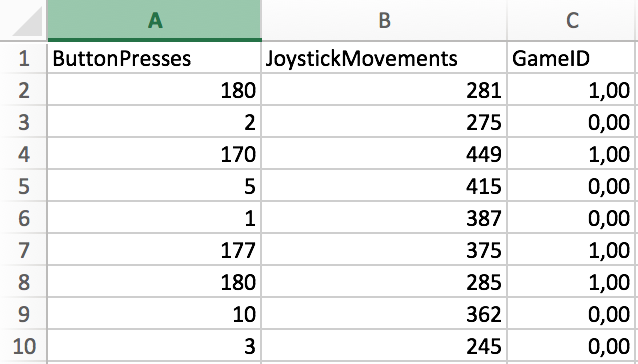
\includegraphics{img/Dataset}
	\caption{Tien voorbeelden van games}
	\label{fig:regressieFig}
\end{figure}


\newpage

\subsection{Logistische regressie}
\label{sec:Logistischeregressie-fase1}

Het eerste algoritme die we gaan testen is logistische regressie. In fase 1 gaan we slecht voorspellingen doen tussen twee verschillende spellen vandaar dat we binaire logistische regressie gaan toepassen die eerder uitgelegd is in sectie \ref{sec:Binaire-logistische-regressie}.

In de code \ref{code:linaireRegressieTweeKlassen} ziet u de implementatie van de binaire logistische regressie. Er worden 2 parameter meegegeven in de functie, input en output. De input is een dubbele array van \textit{double} waarden. Daarin zitten rijen met 2 kolommen die de ButtonPresses en JoystickMovements bevatten. De ouput parameter bevat een enkele array die het GameID bevat. Hoe deze data ingelezen wordt kan u zien in de code \ref{code:dataInlezen}. Met een ExcelReader krijgen we een DataTable die we met de methode ToJagged kunnen omvormen naar ons gewenste dubbele array met de kolomnamen kunnen we de kolommen selecteren. Deze methode is onderdeel van het Accord-framework. 

Wat de LearningRate precies inhoudt wordt later samen met gradient descent uitgelegd (gradient descent zal in het theoretische deel uitgelegd worden)

\subsubsection{Resultaten}
\subparagraph{Snelheid van het algoritme} 
Een eerste belangrijke metric om algortimen te kunnen vergelijken is de snelheid. Het zou niet correct zijn om een stopwatch te laten lopen bij het begin van het programma en te stoppen wanneer het programma klaar is. De tijd om de data in te laden in het programma, de omzetting naar array's, de objecten die worden geïnitialiseerd, ... is allemaal niet zo belangrijk. Wat wel interessant is, is de tijd die het algoritme nodig heeft om tot een hypothese te komen. Dit gebeurt in de \textit{Learn} methode. 
Net voor die lijn code wordt uitgevoerd starten we een stopwatch en erna stoppen we en bekijken het verschil. Omdat de duur verschillend kan zijn nemen we het gemiddelde van 50 metingen. 
Doordat deze dataset slechts 400 voorbeelden bevat en de verschillen tussen de spelletjes Pacman en Mortal Kombat zeer duidelijk zijn heeft het algoritme slecht 1,53842 milliseconden nodig om een hypothese te maken. 
\subparagraph{F-score} (Moet nog theoretisch uitgelegd worden bij methodologie)
\newline
Doordat deze dataset zo simpel is en de testdataset dus ook heeft het algoritme geen probleem om de testdata te classificeren. De precisie is dan ook logischerwijs één en de rappel eveneens.
Zo bekomen we een precisie van 1 die dus wil zeggen dat het algoritme foutloos is op de testdata.  


\textit{Als ik meer data zou voorhanden hebben kan ik de McNeymar's test doen maar in deze fase en deze hoeveelheid data is die test niet echt handig}

%%Logistic regression code
\begin{figure}[]
	\renewcommand{\figurename}{Code}
\begin{lstlisting}
public static void StartLogisticRegression(double[][] input, int[] output)
{
       //LogisticRegression object initialiseren met 2 inputparameters (ButtonPresses & JoystickMovements)
       LogisticRegression logisticRegression = new LogisticRegression()
       {
       		NumberOfInputs = 2
       };
       
      var learner = new LogisticGradientDescent(logisticRegression)
      {
      		LearningRate = 0.0001
      };
     
     // De gradient descent begint met de logistische regressie te optimaliseren
     logisticRegression = learner.Learn(input, output);
}

\end{lstlisting}
\caption{Implementatie binaire logistische regressie}
\label{code:linaireRegressieTweeKlassen}
\end{figure}
%%Data inlezen
\begin{figure}[]
	\renewcommand{\figurename}{Code}
	\begin{lstlisting}
using (var table = new ExcelReader("../../datasetExcel.xls").GetWorksheet("Training"))
   {
       // Convert the DataTable to input and output vectors
       double[][] inputs = table.ToJagged<double>("ButtonPresses", "Joystickmovements");
       int[] outputs = table.Columns["Game"].ToArray<int>();
       
       ...
   }
	\end{lstlisting}
	\caption{Inlezen Excel data}
	\label{code:dataInlezen}
\end{figure}


